\begin{anexosenv}

\partanexos

\chapter{Estrutura}

\begin{figure}[!ht]
	\centering
		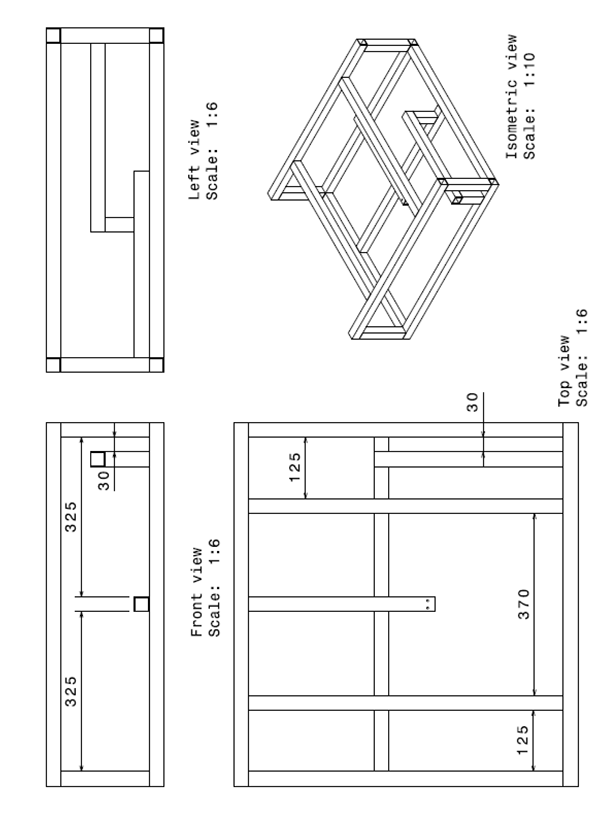
\includegraphics[scale=0.4]{figuras/estrutura/anexos/1(1).png}
	\caption{Estrutura do módulo de seleção e pesagem de garrafas}
\end{figure}

\begin{figure}[!ht]
	\centering
		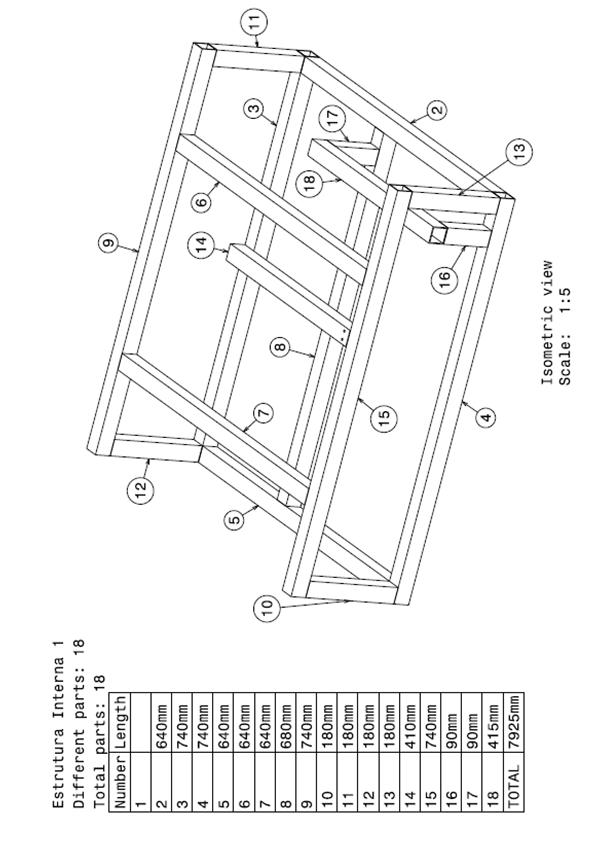
\includegraphics[scale=0.4]{figuras/estrutura/anexos/1(2).png}
	\caption{Estrutura do módulo de seleção e pesagem de garrafas (2)}
\end{figure}

\begin{figure}[!ht]
	\centering
		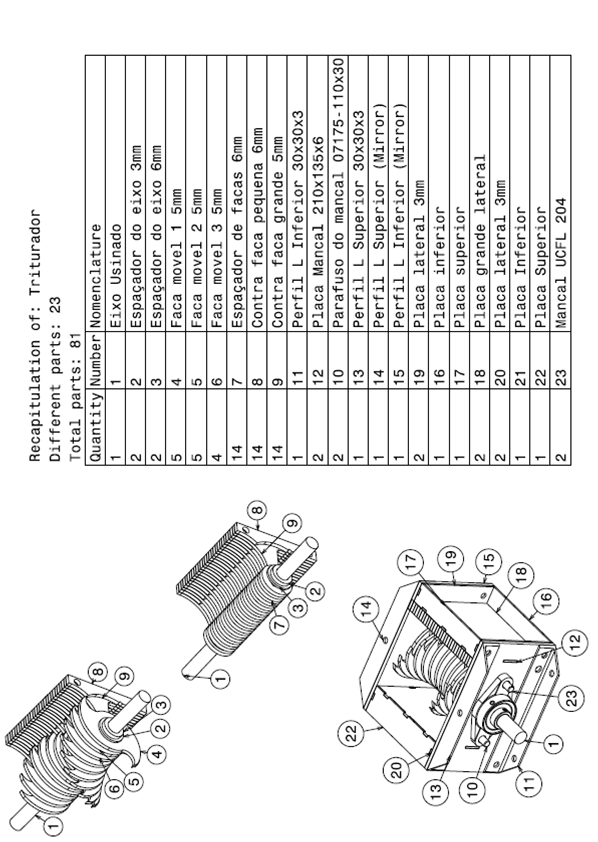
\includegraphics[scale=0.4]{figuras/estrutura/anexos/2.png}
	\caption{Montagem do triturador, com todas as suas partes}
\end{figure}

\begin{figure}[!ht]
	\centering
		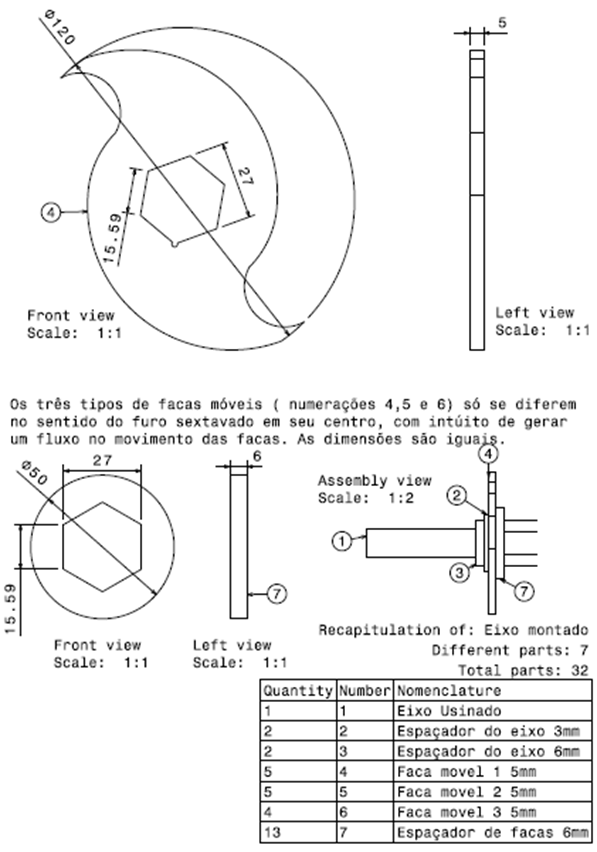
\includegraphics[scale=0.4]{figuras/estrutura/anexos/3.png}
	\caption{Facas móveis e espaçadores}
\end{figure}

\begin{figure}[!ht]
	\centering
		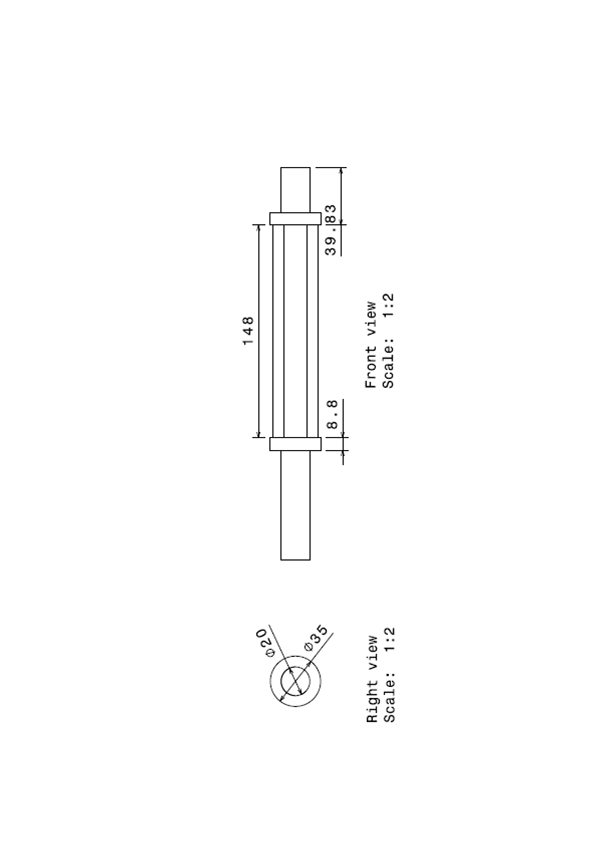
\includegraphics[scale=0.4]{figuras/estrutura/anexos/4.png}
	\caption{Eixo sextavado usinado e arruelas}
\end{figure}

\begin{figure}[!ht]
	\centering
		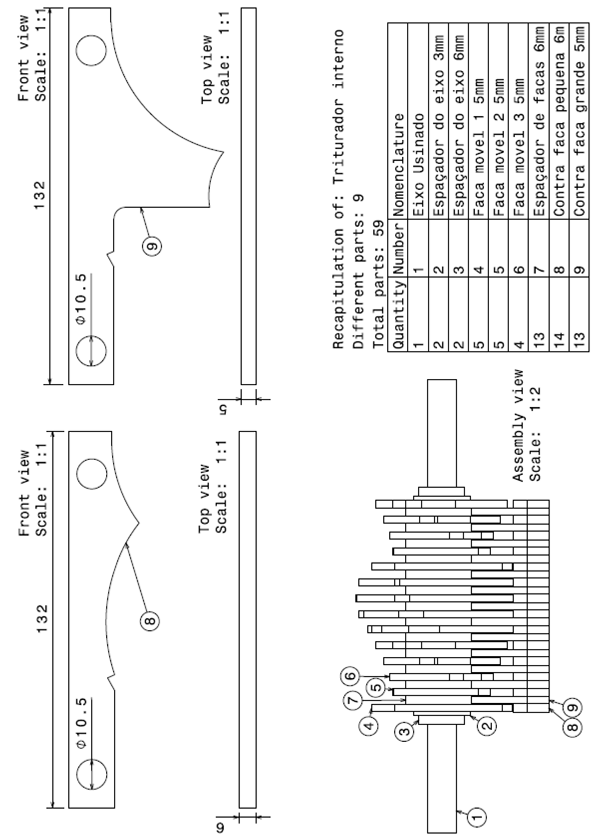
\includegraphics[scale=0.4]{figuras/estrutura/anexos/5.png}
	\caption{Facas fixas e montagem interna do triturador}
\end{figure}

\begin{figure}[!ht]
	\centering
		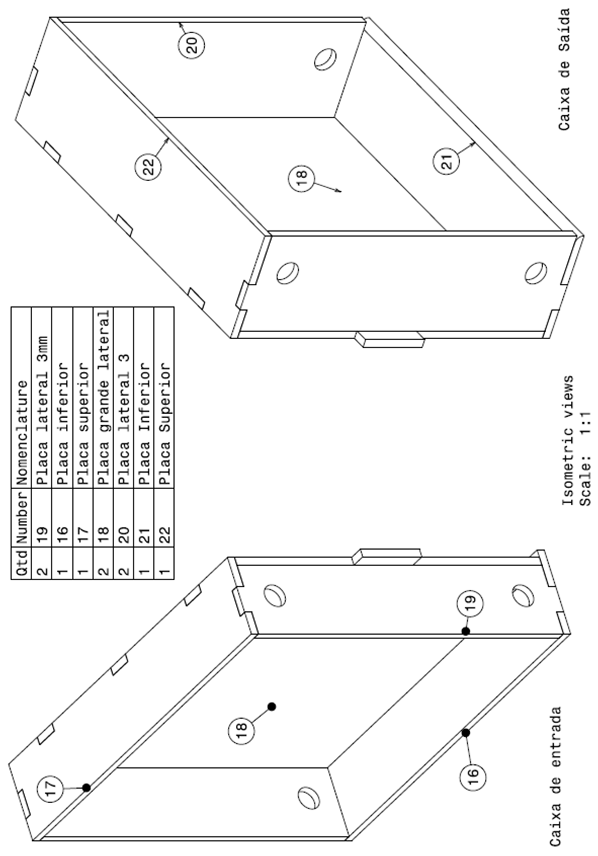
\includegraphics[scale=0.4]{figuras/estrutura/anexos/6.png}
	\caption{Caixas laterais de entrada e de saída}
\end{figure}

\begin{figure}[!ht]
	\centering
		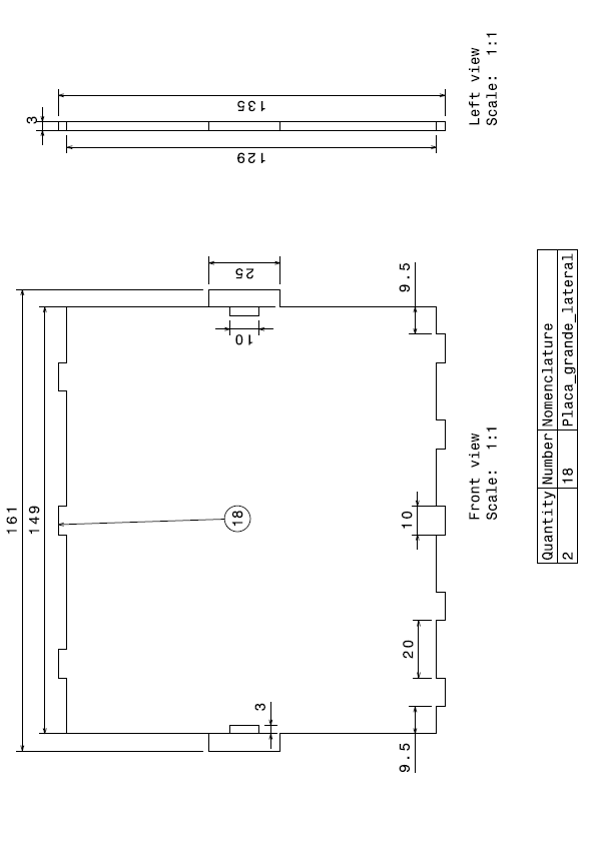
\includegraphics[scale=0.4]{figuras/estrutura/anexos/7.png}
	\caption{Placa maior das caixas laterais}
\end{figure}

\begin{figure}[!ht]
	\centering
		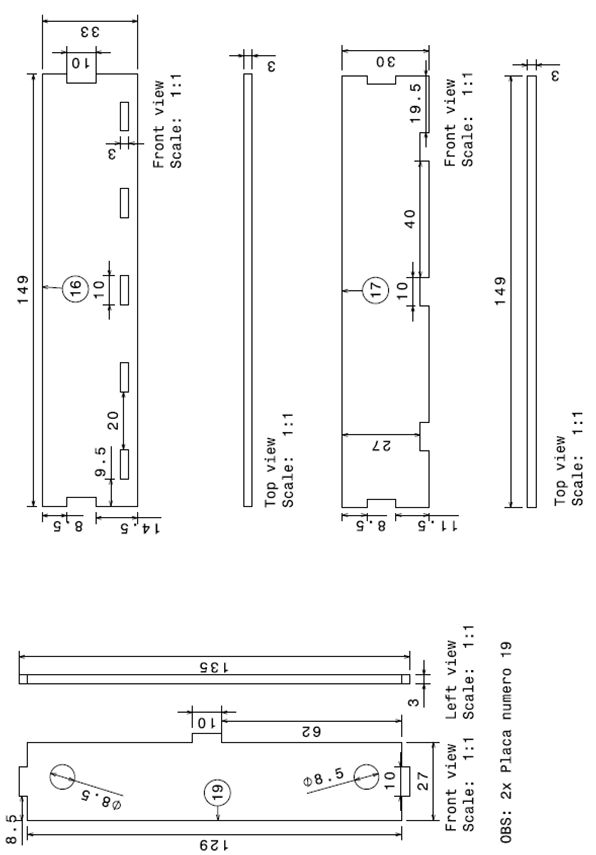
\includegraphics[scale=0.4]{figuras/estrutura/anexos/8.png}
	\caption{Placas menores da caixa lateral de entrada}
\end{figure}

\begin{figure}[!ht]
	\centering
		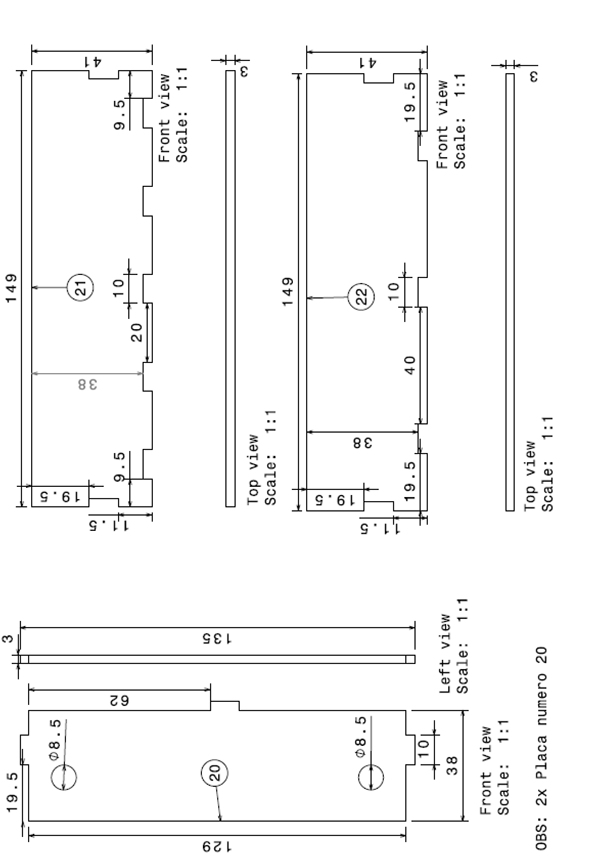
\includegraphics[scale=0.4]{figuras/estrutura/anexos/9.png}
	\caption{Placas menores da caixa lateral de saída}
\end{figure}

\begin{figure}[!ht]
	\centering
		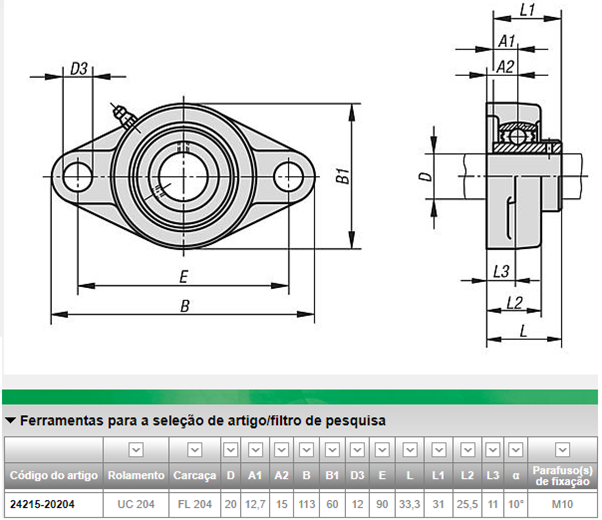
\includegraphics[scale=0.4]{figuras/estrutura/anexos/10.png}
	\caption{Dimensões do Mancal UCFL 204 para o triturador}
\end{figure}

\begin{figure}[!ht]
	\centering
		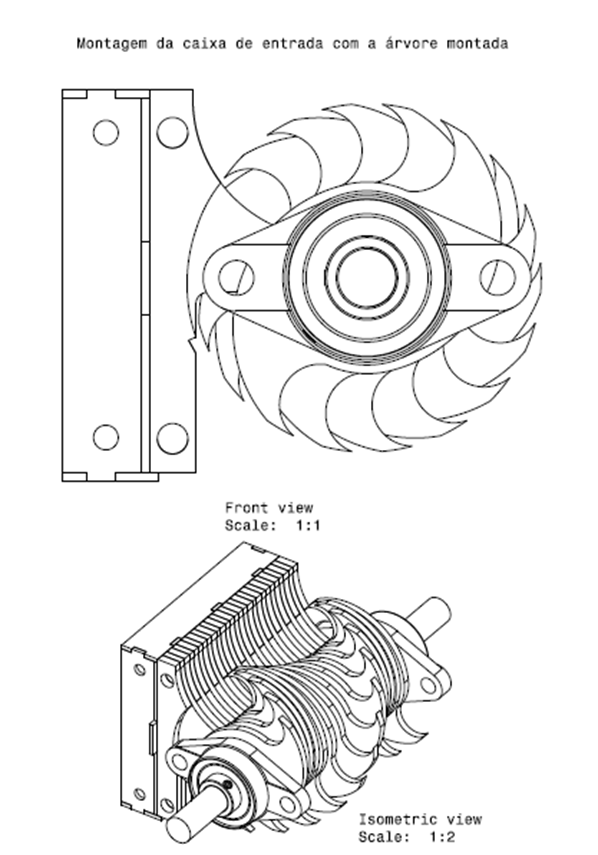
\includegraphics[scale=0.4]{figuras/estrutura/anexos/11.png}
	\caption{Montagem da caixa de entrada com a árvore montada}
\end{figure}

\begin{figure}[!ht]
	\centering
		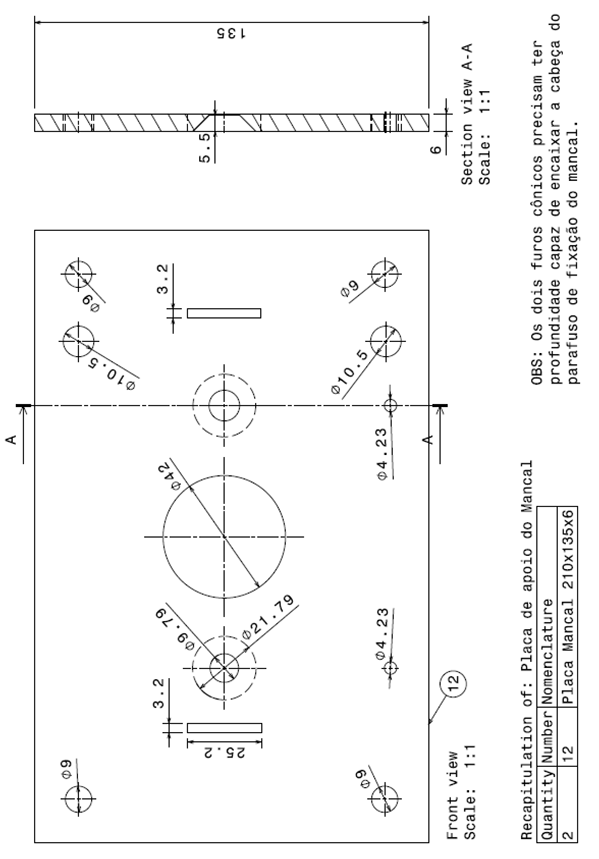
\includegraphics[scale=0.4]{figuras/estrutura/anexos/12.png}
	\caption{Placa de apoio do Mancal}
\end{figure}

\begin{figure}[!ht]
	\centering
		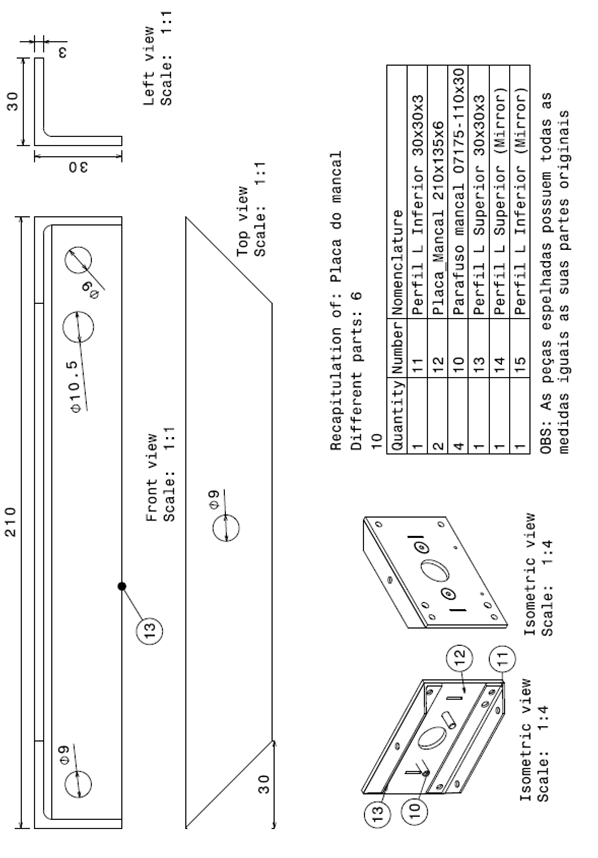
\includegraphics[scale=0.4]{figuras/estrutura/anexos/13.png}
	\caption{Placa de apoio do Mancal}
\end{figure}

\begin{figure}[!ht]
	\centering
		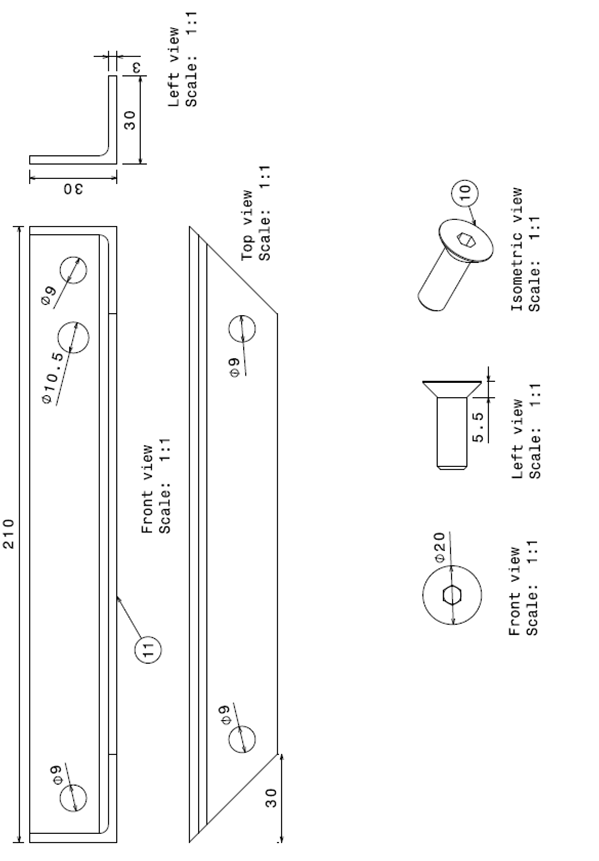
\includegraphics[scale=0.4]{figuras/estrutura/anexos/14.png}
	\caption{Placa de apoio do Mancal}
\end{figure}

\begin{figure}[!ht]
	\centering
		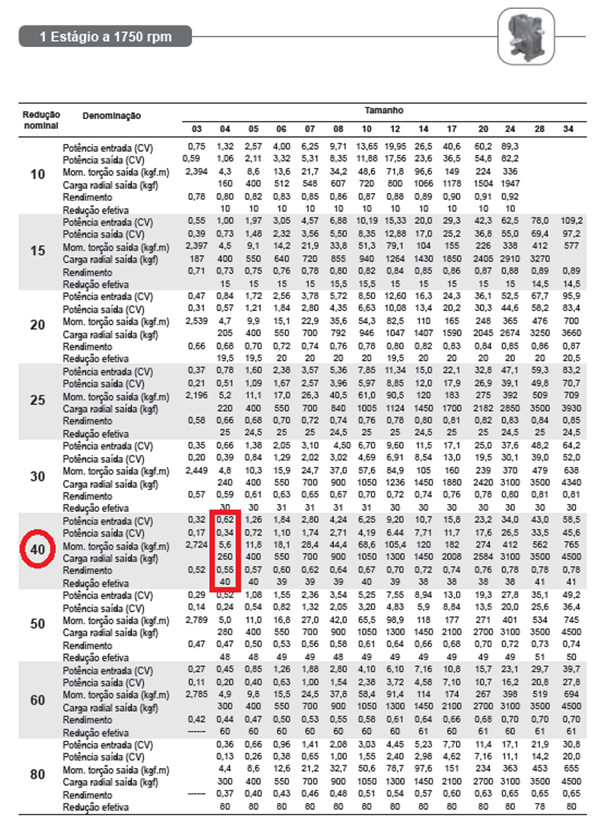
\includegraphics[scale=0.4]{figuras/estrutura/anexos/15.png}
	\caption{Tabela com características do redutor WEG-CESTARI MAGMA-K, redução nominal de 40, tamanho 4}
\end{figure}

\begin{figure}[!ht]
	\centering
		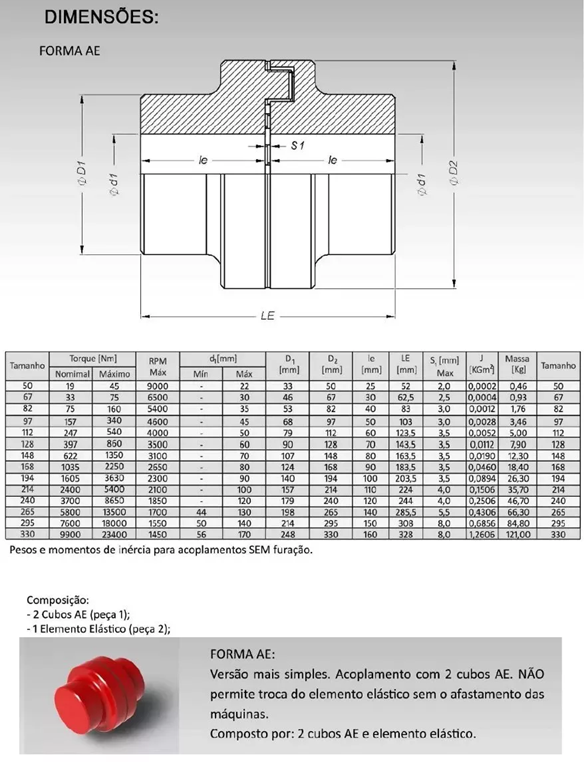
\includegraphics[scale=0.4]{figuras/estrutura/anexos/16.png}
	\caption{Tabela de Acoplamentos Flexíveis Elásticos}
\end{figure}

\begin{figure}[!ht]
	\centering
		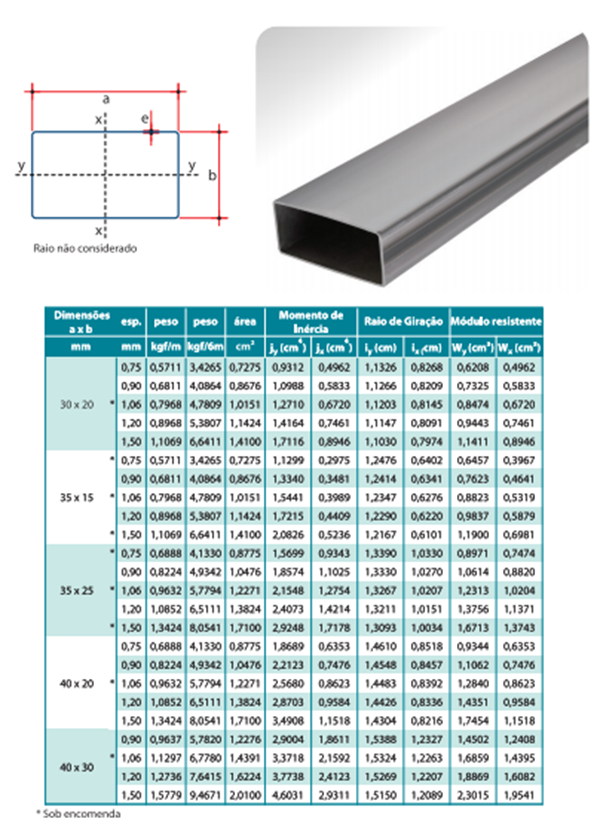
\includegraphics[scale=0.4]{figuras/estrutura/anexos/17.png}
	\caption{Tabela de tubos retangulares}
\end{figure}

\begin{figure}[!ht]
	\centering
		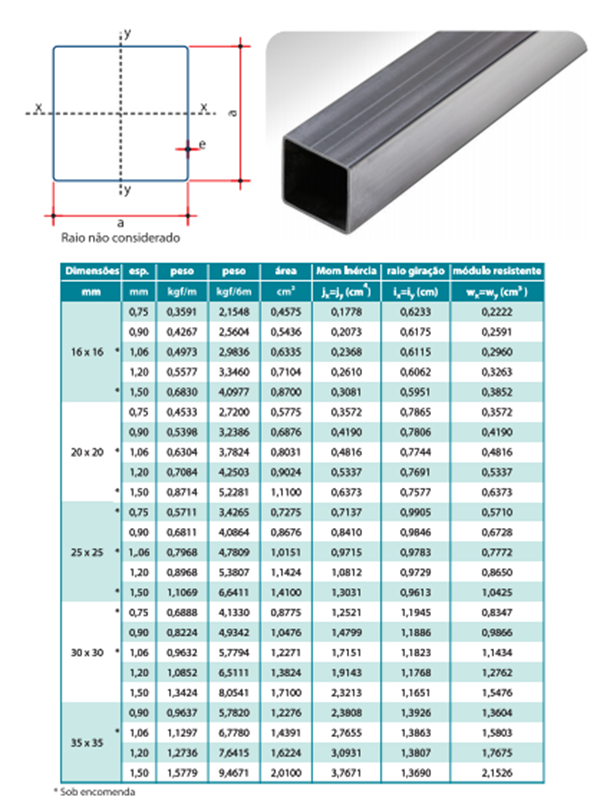
\includegraphics[scale=0.4]{figuras/estrutura/anexos/18.png}
	\caption{Estrutura do módulo de integração}
\end{figure}

\begin{figure}[!ht]
	\centering
		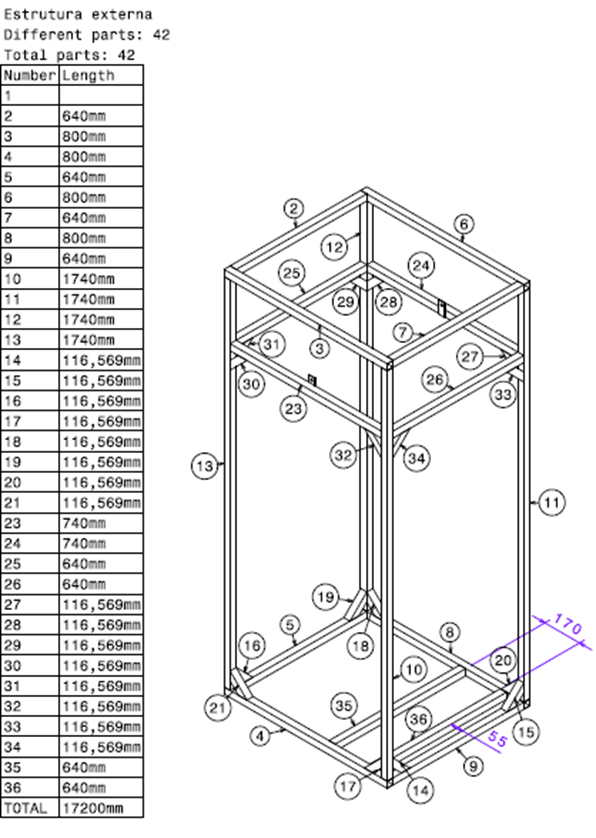
\includegraphics[scale=0.4]{figuras/estrutura/anexos/19.png}
	\caption{Estrutura do módulo de integração}
\end{figure}

\begin{figure}[!ht]
	\centering
		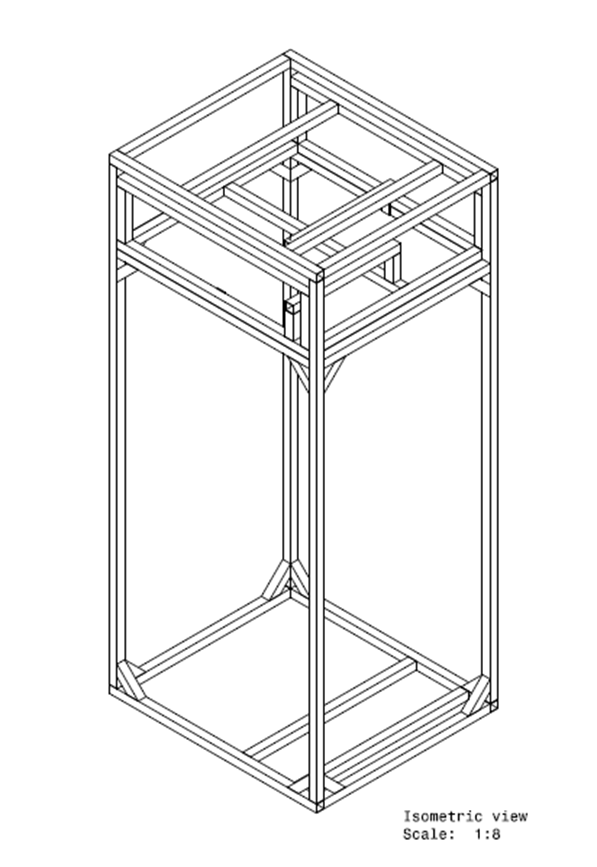
\includegraphics[scale=0.4]{figuras/estrutura/anexos/20.png}
	\caption{Estrutura do módulo de integração com a estrutura do módulo de seleção de garrafas PET}
\end{figure}

\chapter{Segundo Anexo}

Texto do segundo anexo.

\end{anexosenv}

